\section{Ejercicio 1: Crear relaciones - Tarea 2: Relaciones Manuales} 


\begin{enumerate}[1.]

    \item En la Ventana de Power BI Desktop, click en Obtener Datos (Get Data) y luego en Excel.

	\begin{center}
	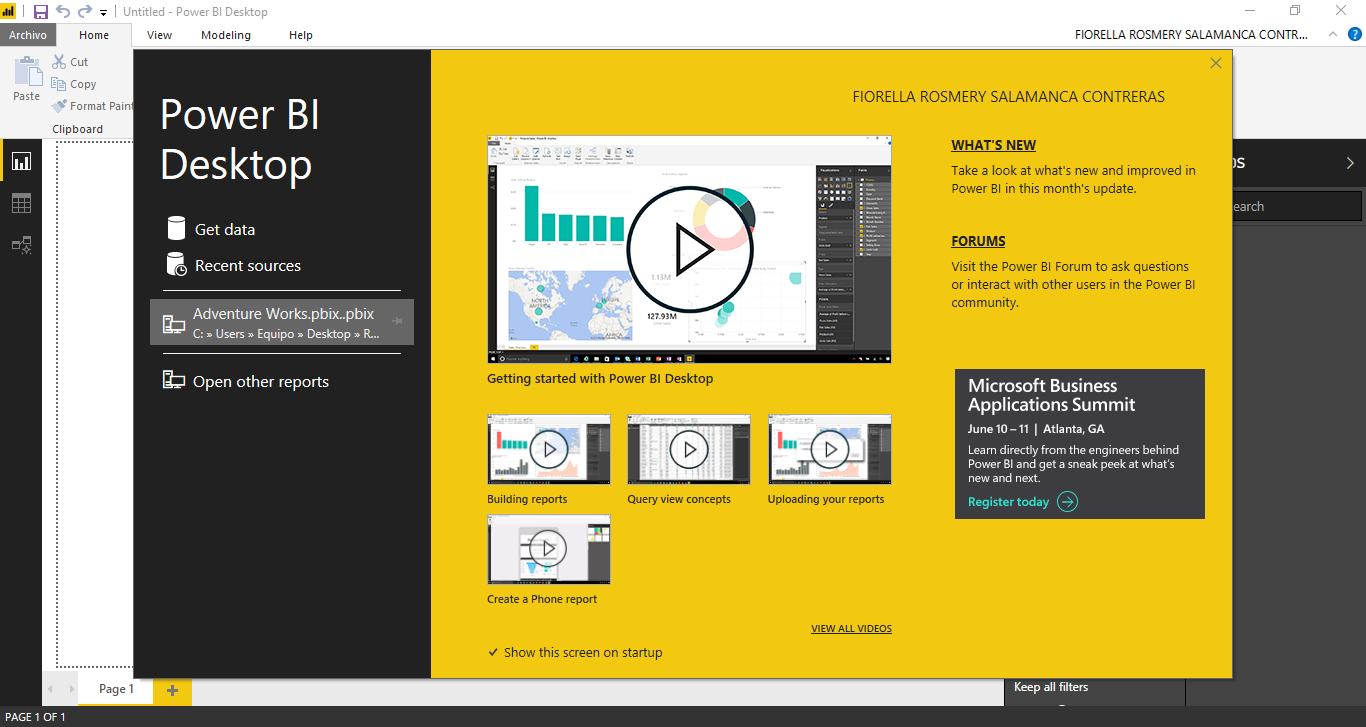
\includegraphics[width=17cm]{./Imagenes/Ejercicio1-Tarea2/1}
	\end{center}	

	\begin{center}
	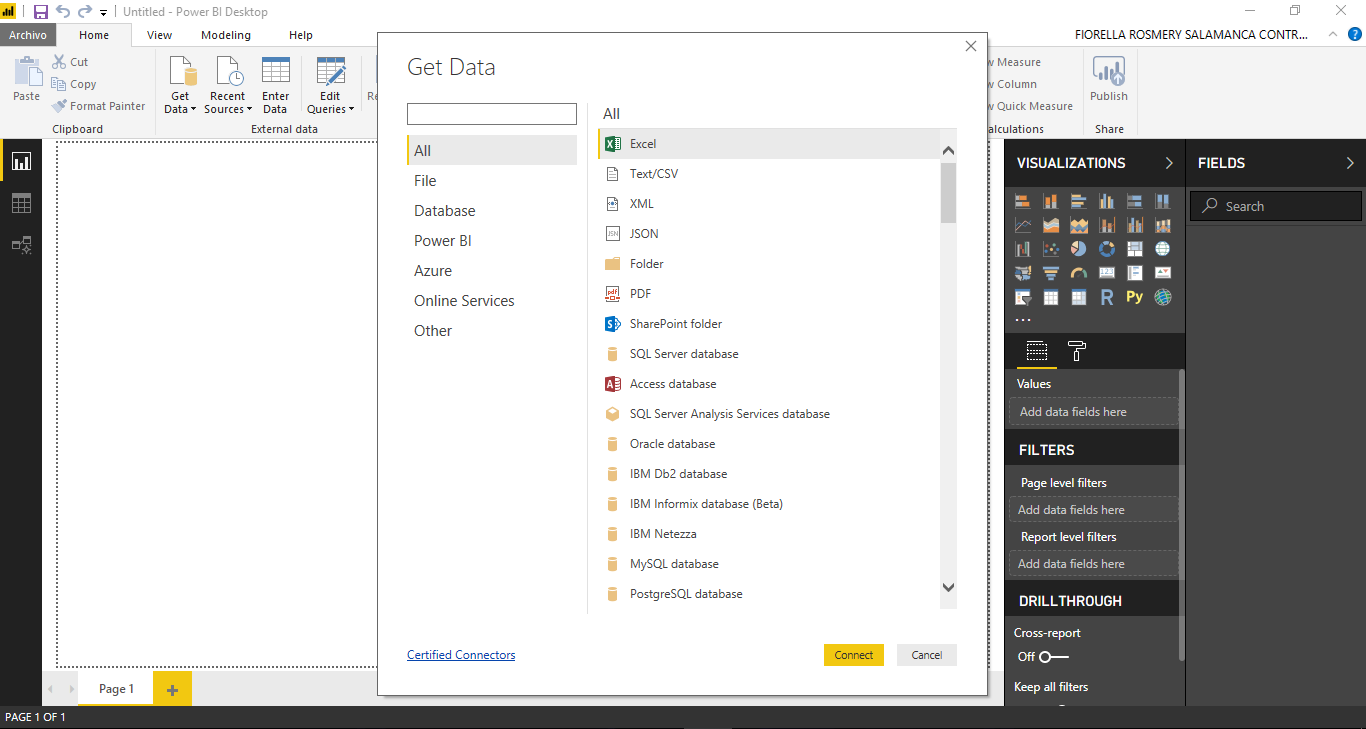
\includegraphics[width=17cm]{./Imagenes/Ejercicio1-Tarea2/2}
	\end{center}	

    \item Abrir el archivo Adventure Works Product Categories.xlsx.

	\begin{center}
	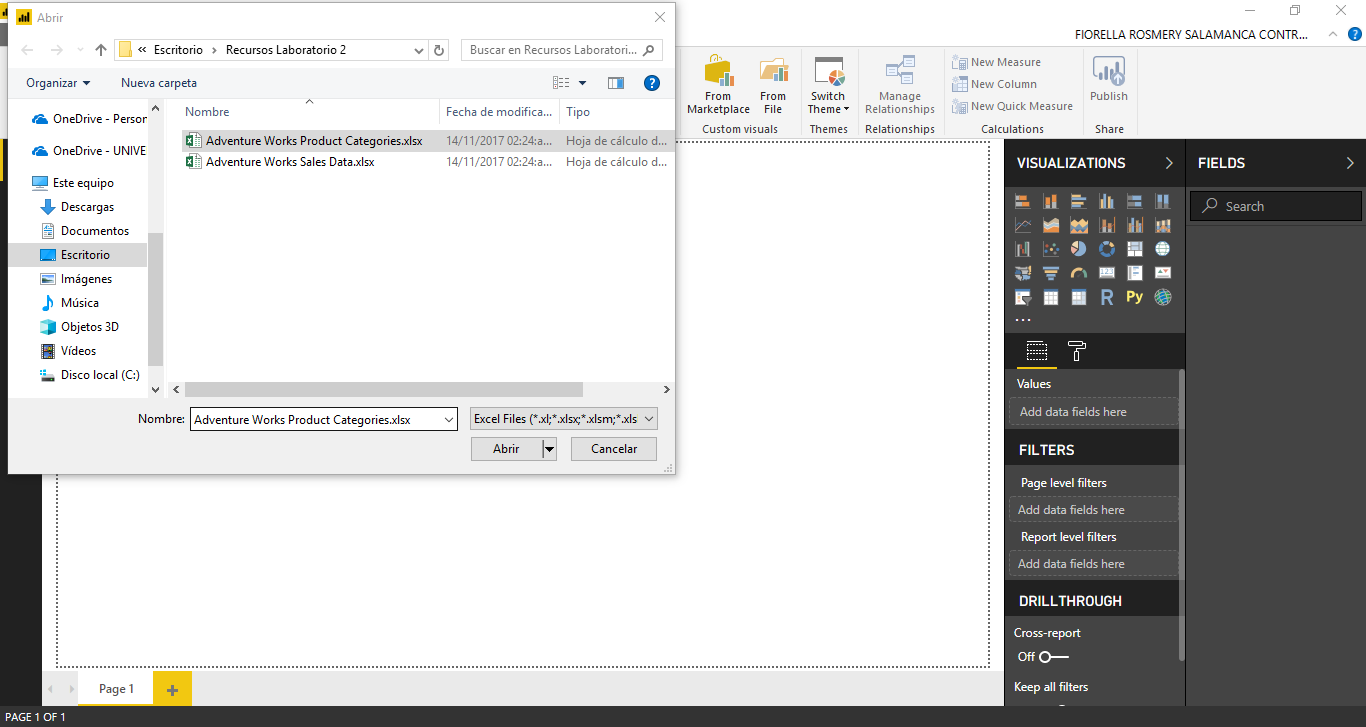
\includegraphics[width=17cm]{./Imagenes/Ejercicio1-Tarea2/3}
	\end{center}	

    \item En el cuadro de dialogo Explorador (Navigator), seleccionar las hojas DimProductCategory, and DimProductSubcategory, y luego hacer click en Cargar (Load).

	\begin{center}
	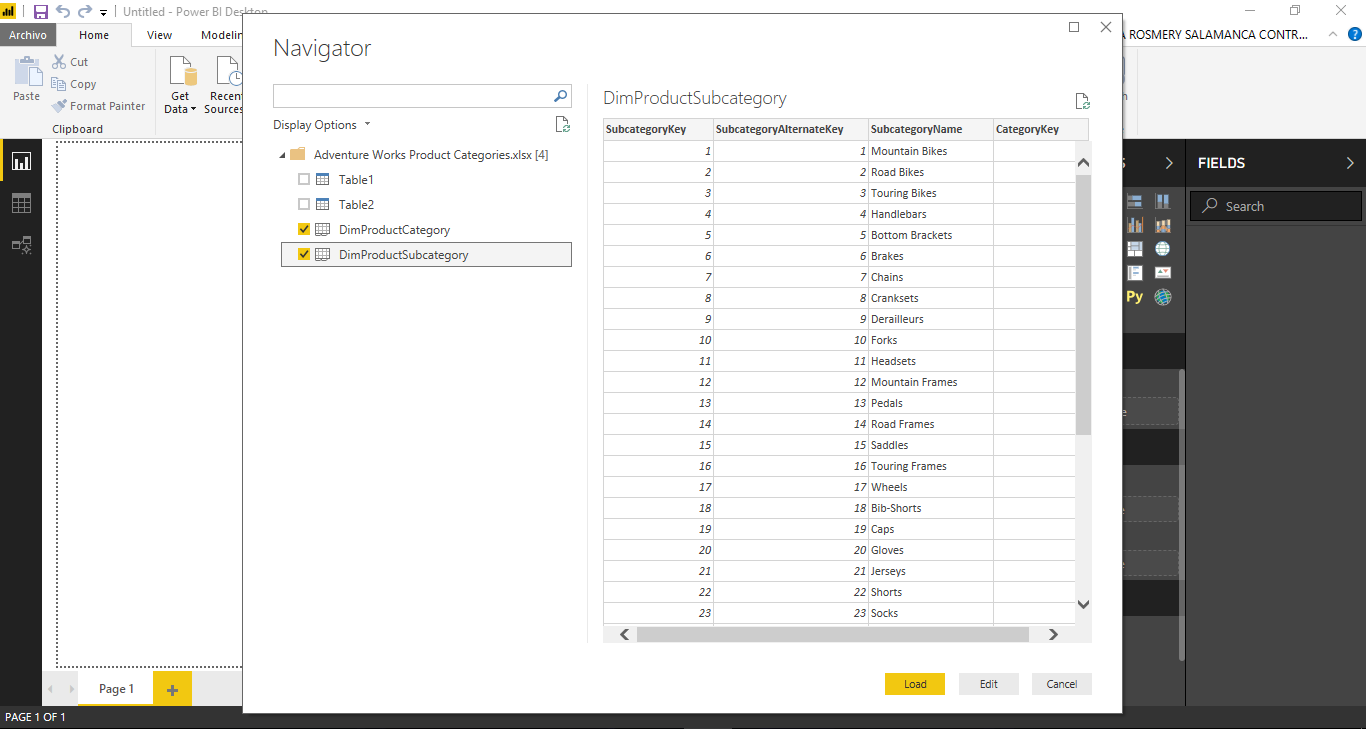
\includegraphics[width=17cm]{./Imagenes/Ejercicio1-Tarea2/4}
	\end{center}	

    \item  En el panel de Relaciones, revisar la relación que Power BI ha creado entre las dos tablas.

	\begin{center}
	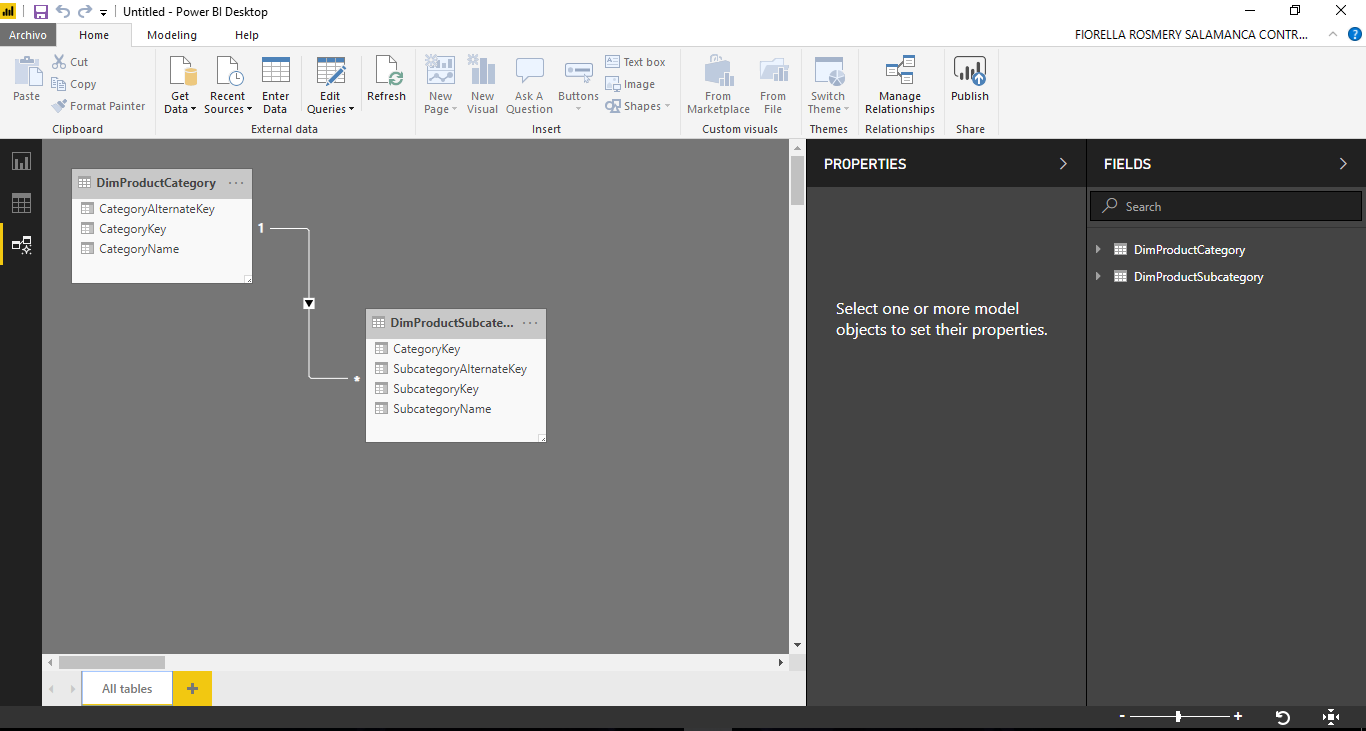
\includegraphics[width=17cm]{./Imagenes/Ejercicio1-Tarea2/5}
	\end{center}	

    \item Hacer click en la línea de la relación entre DimProductCategory, y DimProductSubcategory, y seleccionar Eliminar (Delete).
    \item En el cuadro de dialogo Eliminar relación (Delete Relationship), hacer click en Borrar (Delete).

	\begin{center}
	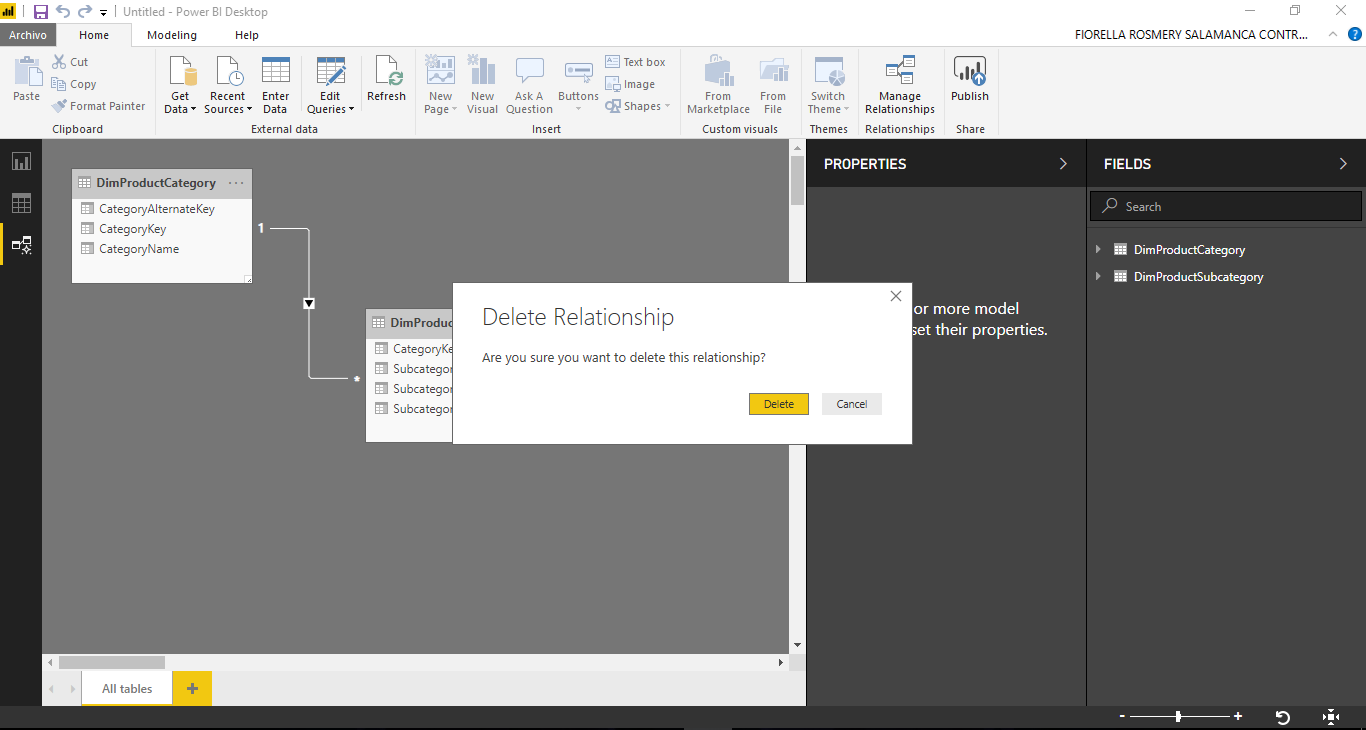
\includegraphics[width=17cm]{./Imagenes/Ejercicio1-Tarea2/6}
	\end{center}	

    \item Arrastrar la columna CategoryKey en la tabla DimProductSubcategory a la columna Category en la tabla DimProductCategory, para crear una relación Muchos a uno (Many to One (*:1)), y una dirección de filtro cruzado (Cross filter direction) en ambos.

	\begin{center}
	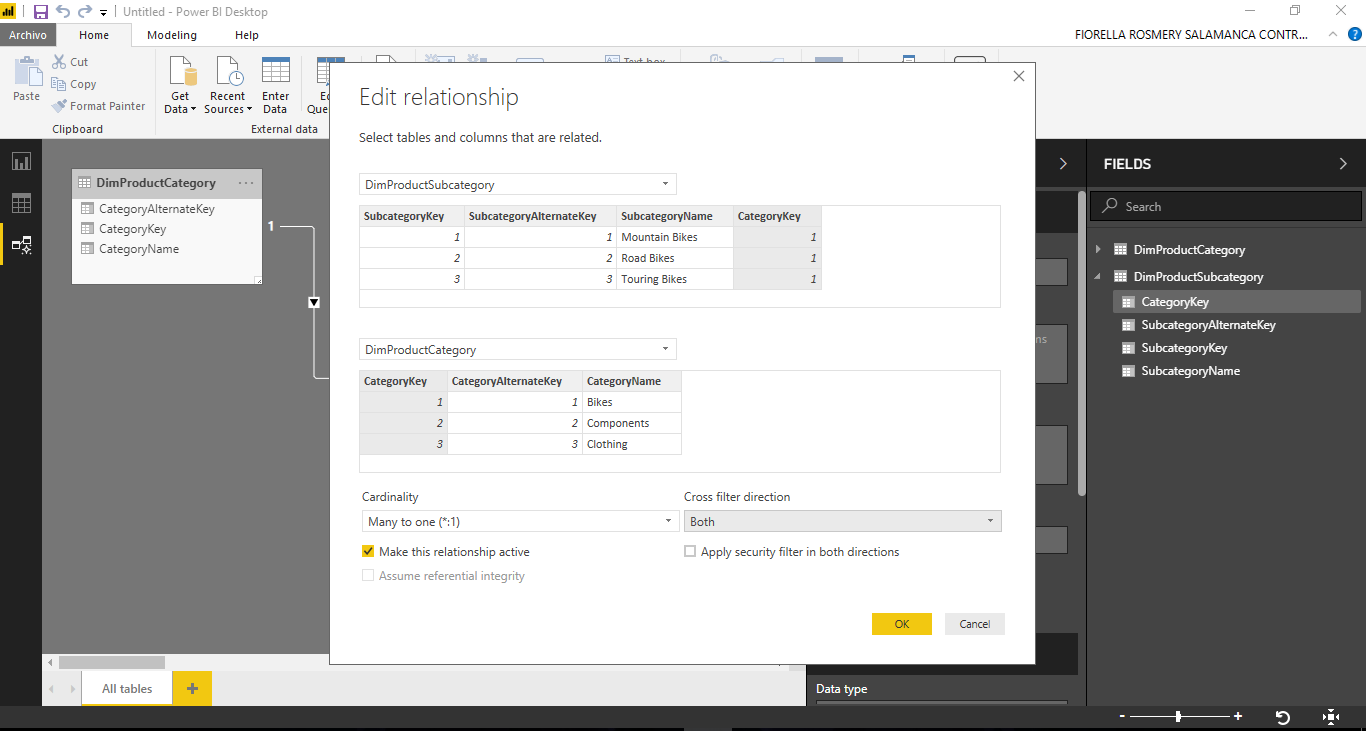
\includegraphics[width=17cm]{./Imagenes/Ejercicio1-Tarea2/7}
	\end{center}	

    \item En la tabla DimProduct, arrastrar la columna ProductSubcategoryKey a la columna SubcategoryKey en la tabla DimProductSubcategory, para crear una relación de Muchos a Uno (Many to One (*:1)), y una dirección de filtro cruzado (Cross filter direction) en ambos.

	\begin{center}
	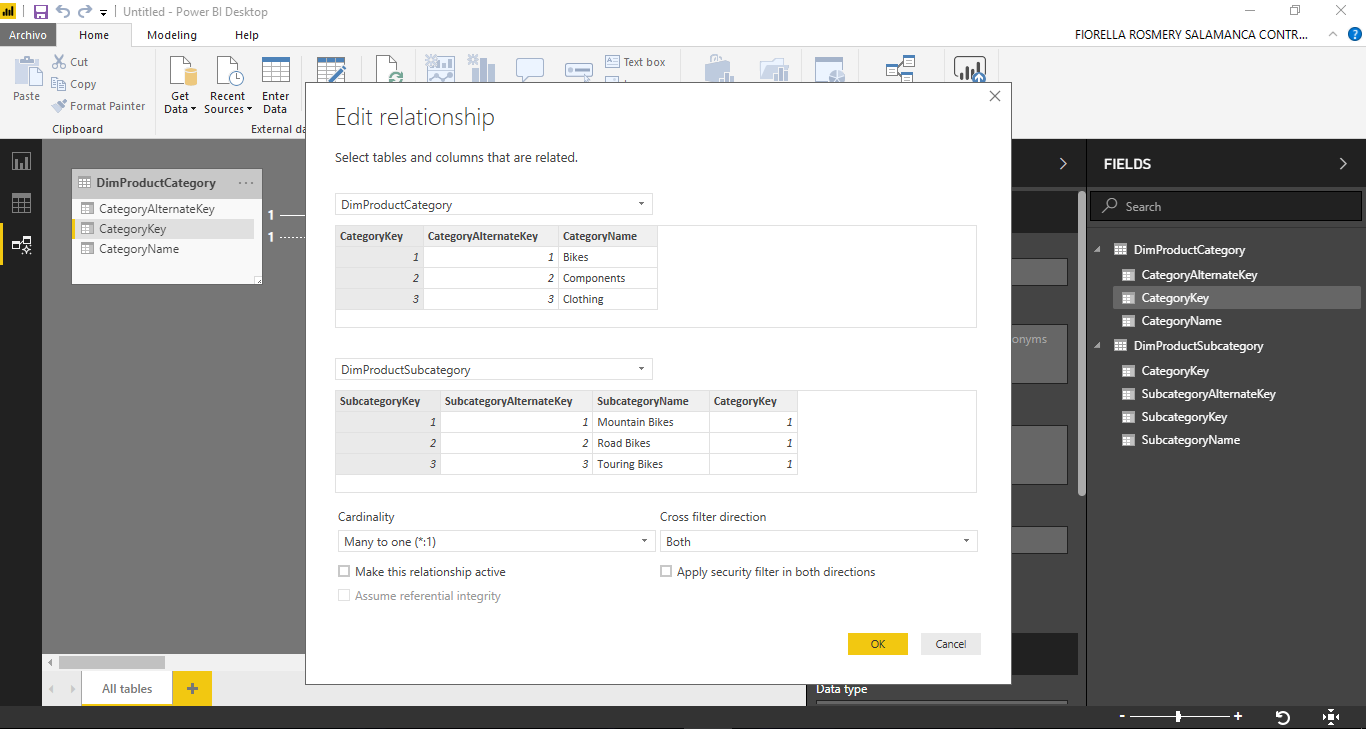
\includegraphics[width=17cm]{./Imagenes/Ejercicio1-Tarea2/8}
	\end{center}	

	\begin{center}
	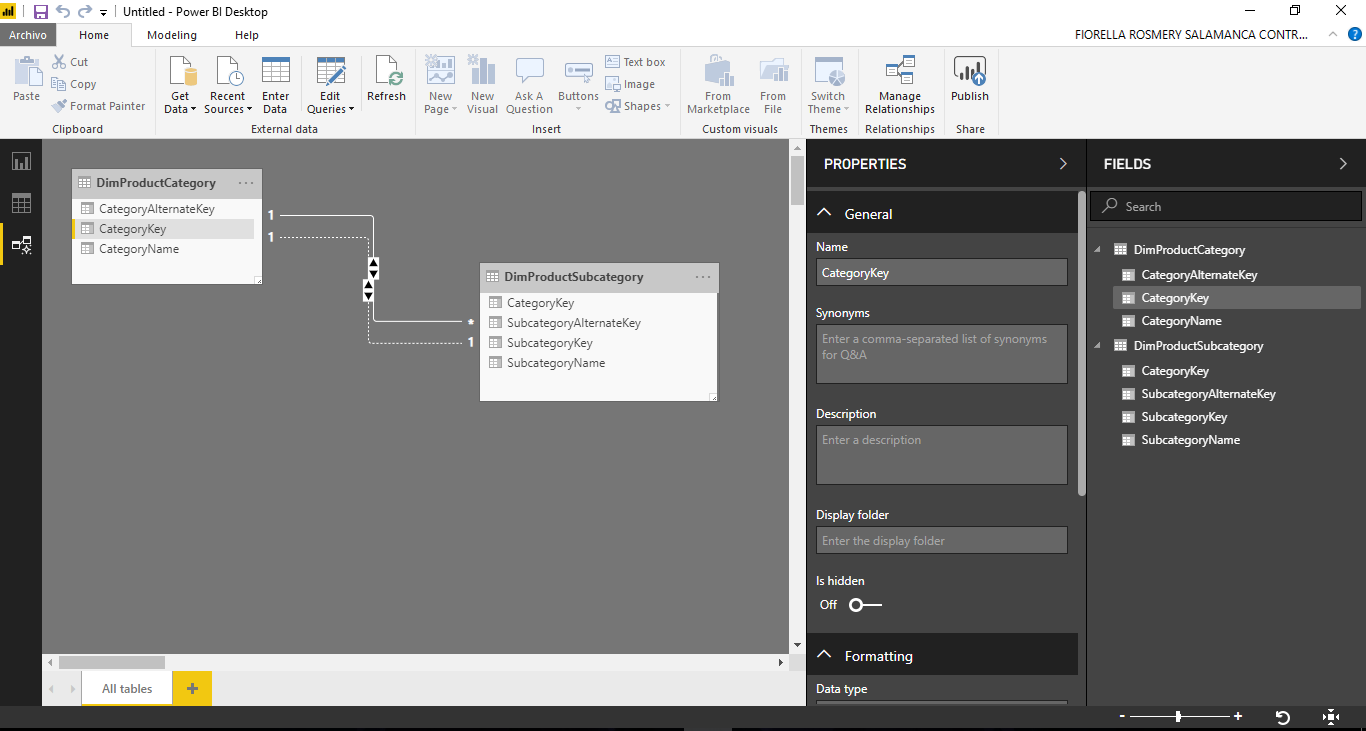
\includegraphics[width=17cm]{./Imagenes/Ejercicio1-Tarea2/9}
	\end{center}	

    \item Hacer click en Guardar.

\end{enumerate}


